%; whizzy chapter
% -initex iniptex -latex platex -format platex -bibtex jbibtex -fmt fmt
% 以上 whizzytex を使用する場合の設定。

%     Tokyo Debian Meeting resources
%     Copyright (C) 2011 Junichi Uekawa

%     This program is free software; you can redistribute it and/or modify
%     it under the terms of the GNU General Public License as published by
%     the Free Software Foundation; either version 2 of the License, or
%     (at your option) any later version.

%     This program is distributed in the hope that it will be useful,
%     but WITHOUT ANY WARRANTY; without even the implied warranty of
%     MERCHANTABILITY or FITNESS FOR A PARTICULAR PURPOSE.  See the
%     GNU General Public License for more details.

%     You should have received a copy of the GNU General Public License
%     along with this program; if not, write to the Free Software
%     Foundation, Inc., 51 Franklin St, Fifth Floor, Boston, MA  02110-1301 USA

%  preview (shell-command (concat "evince " (replace-regexp-in-string "tex$" "pdf"(buffer-file-name)) "&"))
% 画像ファイルを処理するためにはebbを利用してboundingboxを作成。
%(shell-command "cd image201101; ebb *.png")

%%ここからヘッダ開始。

\documentclass[mingoth,a4paper]{jsarticle}
\usepackage{monthlyreport}

% 日付を定義する、毎月変わります。
\newcommand{\debmtgyear}{2011}
\newcommand{\debmtgmonth}{4}
\newcommand{\debmtgdate}{16}
% (+ (* (- 2010 2005) 12) 10) started from zero
\newcommand{\debmtgnumber}{75}

\begin{document}

\begin{titlepage}
\thispagestyle{empty}
% タイトルページ:編集必要な部分は最初のマクロに飛ばすこと

\vspace*{-2cm}
第\debmtgnumber{}回 東京エリア Debian 勉強会資料\\
\hspace*{-2cm}

\includegraphics[width=210mm]{image201003/debsen.eps}\\
\hfill{}\debmtgyear{}年\debmtgmonth{}月\debmtgdate{}日

% ここはアップデートすること
\rotatebox{10}{\fontsize{32}{32} {\gt 特集1: backports.debian.org の活用}}

\rotatebox{10}{\fontsize{32}{32} {\gt 特集2: initram-toolsの使い方}}

\vspace*{-2cm}
\hfill{}
\includegraphics[height=6cm]{image200502/openlogo-nd.eps}
\end{titlepage}

\dancersection{Introduction}{上川 純一}

\begin{multicols}{2}
 

 今月のDebian勉強会へようこそ。これからDebianの世界にあしを踏み入れると
 いう方も、すでにどっぷりとつかっているという方も、月に一回Debianについ
 て語りませんか?

 Debian勉強会の目的は下記です。

 \begin{itemize}
 \item \underline{Debian Developer} (開発者)の育成。
 \item 日本語での「\underline{開発に関する情報}」を整理してまとめ、アップデートする。
 \item \underline{場}の提供。
 \begin{itemize}
  \item 普段ばらばらな場所にいる人々が face-to-face で出会える場を提供
	する。
  \item Debian のためになることを語る場を提供する。
  \item Debianについて語る場を提供する。
 \end{itemize}
 \end{itemize}		

 Debianの勉強会ということで究極的には参加者全員がDebian Packageをがりがり
 と作るスーパーハッカーになった姿を妄想しています。情報の共有・活用を通し
 て Debianの今後の能動的な展開への土台として、「場」としての空間を提供す
 るのが目的です。

\end{multicols}

\newpage

\begin{minipage}[b]{0.2\hsize}
 \definecolor{titleback}{gray}{0.9}
 \colorbox{titleback}{\rotatebox{90}{\fontsize{80}{80} {\gt デビアン勉強会} }}
\end{minipage}
\begin{minipage}[b]{0.8\hsize}
\hrule
\vspace{2mm}
\hrule
\begin{multicols}{2}
\tableofcontents
\end{multicols}
\vspace{2mm}
\hrule
\end{minipage}

\dancersection{事前課題}{上川 純一}

今回の事前課題は以下です:
\begin{enumerate}
 \item 今回の震災でDebianをどのように活用してますか。
\end{enumerate}
この課題に対して提出いただいた内容は以下です。
\begin{multicols}{2}
{\small
%; whizzy-master ../debianmeetingresume201101.tex
% $B0J>e$N@_Dj$r$7$F$$$k$?$a!"$3$N%U%!%$%k$G(B M-x whizzytex $B$9$k$H!"(Bwhizzytex$B$,MxMQ$G$-$^$9!#(B


\begin{prework}{ $B5HLn(B(yy\_y\_ja\_jp) }

$BIaCJDL$j%G%9%/%H%C%W4D6-$H$7$F;H$C$F$^$9!%(B
\end{prework}

\begin{prework}{ henrich }

$B3hMQ$OFCCJ$7$F$$$^$;$s!#DdEE$N$?$a$K2H%5!<%P$HCN?M$N2q<R$KCV$$$F$"$k%5!<%P$NN>J}$,;_$^$C$FFq57$7$^$7$?!#(B
\end{prework}

\begin{prework}{ dictoss($B?yK\!!E5=<(B) }

 \begin{itemize}
  \item $BDdEE$G(BPC$B$r5/F0$G$-$J$$$H$-$b$"$j!"$`$7$m(BDebian$B$r;H$($J$$$H$-$b$"$j$^$7$?!#(B
  \item $B;H$$J}$O%a!<%k$7$?$j!"(BWeb$B%V%i%&%:$r$7$?$j$HIaCJ$HJQ$o$i$J$$46$8$G(B
	$B$9!#(B
 \end{itemize}
\end{prework}

\begin{prework}{ $B4d>>(B $B?.MN(B }

 \begin{itemize}
  \item chromium $B$N3HD%%W%m%0%i%`$r=q$$$F!"CO?L$,Mh$?$i%&%#%s%I%&$r=P$9$h$&$J%W%m%0%i%`$r=q$$$F$_$^$7$?!#(B
  \item $BDdEEMQ$K(BVPS$B$r7@Ls$7$F!"(BDebian$B$K$7$?!#(B
  \item Debian$B>e$G(BOSM$B$r$$$8$C$?$j$7$?!#(B
 \end{itemize}
 
\end{prework}

\begin{prework}{ $BLnEg!!5.1Q(B }

$B?L:R$GBgJQ$JCf!"Hs>o$K$D$^$i$J$$Nc$GCQ$:$+$7$$$N$G$9$,!"(B

 \begin{enumerate}
  \item $B?L:R>pJs=8$a$O<g$K(Bdebain+ephipany$B$NAH$_9g$o$;$,B?$$$G$9(B
  \item $B?L:R$K4X$9$k=t!9$N>pJs=8$a$G(BNIKKEINET($BM-NA!K$rMxMQ$9$k:]$O(Bdebian+iceweasel$B$P$+$j$G$9!#(B
  \item USB$B%V!<%H2DG=$J%Q%=%3%s$5$($"$l$PM-;v$N:]$I$3$G$bBP1~$G$-$k$h$&(B
	$B$K<+J,$N(Bdebian$B4D6-$rF~$l$?%V!<%H2DG=$J(BUSB$B%a%b%j$r;}$AJb$$$F$$$?(B
	$B$j$7$^$9!#<+M3$J;H$$J}$G$-$k<+J,$N4D6-$r%]%1%C%H$K$7$N$P$;$F;}$A(B
	$BJb$1$k$N$O$h$$$+$b!#CO?L$"$C$?$H$-$O$3$N(BUSB$B$r6;%]%1%C%H$KF~$l$F(B
	$BHrFq$7$^$7$?!#!J$?$^$?$^F~$C$F$$$?$H$b$$$&!#$G$b<+J,$N4D6-$O$3$3(B
	$B$K$"$k$+$i$H$A$g$C$H0B?4$G$-$?$N$O3N$+!#!K(B
 \end{enumerate}
 $B"(JL$K(Bdebian$B$G$J$/$F$b$h$$$8$c$s$H$$$&%D%C%3%_$O%J%7$NJ}8~$G!#(B
\end{prework}

\begin{prework}{ $B;3ED(B }

$B?L:R4X78$@$H$"$^$j3hLv$7$F$$$J$$$G$9!D(B

$B:#2s$O(BPC$B$r;}$C$FHo:R$7$?$b$N$N$[$H$s$I=PHV$,$J$/!"(B
$B7HBSEEOC$@$1$,3hLv$7$^$7$?!#(B

$B$=$&$$$&$o$1$G!"Aa5^$K(BAndroid$B7HBS$K(BDebian/Ubuntu$B$r(B
$BF~$l$?$$$H;W$$$^$9!J(BiDroid$B$GDLOC$G$-$k$N$@$m$&$+!)!K!#(B
\end{prework}

\begin{prework}{ $BB<ED?.?M(B }

$B?L:R$KBP$7$FD>@\$O3hMQ$G$-$F$$$^$;$s!#$?$@!"(BSahana Eden$B$NF|K\%A!<%`$N(BLaunchpad, Bazaar$B$KBP$9$k5?Ld$KEz$($k$3$H$G4V@\E*$K9W8%$G$-$l$P$H!#(B
\end{prework}

\begin{prework}{ Kiwamu Okabe }

sakura VPS$B>e$K(BDebian$B$r%$%s%9%H!<%k$7$F$$$^$9!#(B
$B;E;v$G(BNetBSD$B$r;H$C$?3+H/$r$7$F$$$k$N$G$9$,%M%C%H%o!<%/$,;_$^$C$F$b%a%s%P!<$,3+H/7QB3$G$-$k$h$&$K8x<0(Bcvs$B%j%]%8%H%j$N(Btar$B6L$r<h$k$h$&$K$7$^$7$?!#(B

netbsd\_cvs =rsync=$>$ sakura\_vps(debian) =tar$B6L(B=$>$ $B2q<R$N%a%s%D(BPC

http://www.masterq.net/files/
$BKhD+(B4$B;~$4$m99?7$7$F$$$^$9!#(B
\end{prework}

\begin{prework}{ Osamu MATSUMOTO }

$BL$Dj$@$C$?$N$G2sEz$J$7$G!#(B
$B$b$&(B10$BG/$0$i$$(BDebian$B;H$C$F$P$+$j$J$N$G!"9W8%$7$?$$$H;W$C$F$$$k!#(B
\end{prework}

\begin{prework}{ yamamoto }

$B:#2s$N?L:R$G5"Bp;~4V$,Aa$/$J$C$?J,!"%^%7%s$X$N$*?($j$,A}$($^$7$?!#(B
$B:#$b$*$$$i$N2#$G%&%s%&%sS9$C$F$$$^$9!#(B
\end{prework}

\begin{prework}{ $B$^$($@$3$&$X$$(B }

$B2f$,2H$N(BDebian$B%^%7%s$?$A!#(B
\begin{itemize}
 \item $BCO?L$NEvF|!"%h%a$H%G%#%:%K!<%7!<$+$i5"$l$J$/!"MbF|5"Bp$9$k$^$G(B
       $B$3$^$a$,?4G[$G;EJ}$J$+$C$?$N$G!"(BOpenBlockS 600$B$K(BWeb$B%+%a(B
       $B%i$r$D$1$F!"$3$^$A$c$s4F;k%7%9%F%`$r:n$j$^$7$?!#IaCJ$NMM;R$d!"Dd(B
       $BEE$N3NG'!"Bg$-$JM>?L$,$"$C$?:]$N<+Bp$NMM;R$r8+$F$^$9!#(B
 \item $B0lJ}!"(BOpenBlockS 266$B$G%O!<%I%G%#%9%/$G2TF/$7$F$$$?IaDL$N%5!<%P$?$A(B(Web,
       DNS, CouchDB, Git$B%j%b!<%H%j%]%8%H%jMQ(B, $B4F;k$J$I(B)$B$O!"DdEE$KHw$($9(B
       $B$Y$FDd;_$7$^$7$?!#(B
 \item $BCO?L$ND>8e$O$7$P$i$/(BMacBook$B$N;HMQ$O95$($F!"(BiPad$B$d(BAndroid$B;H$C$F$^(B
       $B$7$?!#(B
 \item $B:#8e$O30$K=P$;$k%5!<%P$d%G!<%?$O!"4pK\%/%i%&%I%5!<%S%9$rMxMQ$7$F!"(B
       OpenBlockS$BEy$O%G%#%9%/%l%92=$7$F!"%;%s%5!<$G$N4F;k@lMQ$K$7$F$$$/(B
       $BM=Dj$G$9!#(B
\end{itemize}

\end{prework}

}
\end{multicols}

\dancersection{最近のDebian関連のミーティング報告}{上川純一}
\subsection{東京エリアDebian勉強会74回目報告}

% (query-replace-regexp "<.*?>" "")
% (query-replace-regexp "^[	 ]\+" "")

三月はOSC 2011 Tokyo/Springでのセミナー、およびブース展示を行いました。
午前中にGPG/CACertキーサインパーティ、午後は山田さん中心でCACert公式トレー
ニングも開催されました。


\dancersection{Debian Trivia Quiz}{上川 純一}

ところで、みなさん Debian 関連の話題においついていますか?Debian関連の話
題はメーリングリストをよんでいると追跡できます。ただよんでいるだけではは
りあいがないので、理解度のテストをします。特に一人だけでは意味がわからな
いところもあるかも知れません。みんなで一緒に読んでみましょう。

今回の出題範囲は\url{debian-devel-announce@lists.debian.org} や \url{debian-devel@lists.debian.org}に投稿された
内容とDebian Project Newsからです。

\begin{multicols}{2}
%; whizzy-master ../debianmeetingresume201101.tex
% $B0J>e$N@_Dj$r$7$F$$$k$?$a!"$3$N%U%!%$%k$G(B M-x whizzytex $B$9$k$H!"(Bwhizzytex$B$,MxMQ$G$-$^$9!#(B
%
% $B$A$J$_$K!"%/%$%:$OJL%V%i%s%A$G:n@.$7!"$N$A$K%^!<%8$7$^$9!#5U$K%^!<%8$7(B
% $B$J$$$h$&$K$7$^$7$g$&!#(B
% (shell-command "git checkout quiz-prepare")

\santaku
{2011$BG/EY(B Debian JP $B2qD9$OC/$G$7$g$&$+!)(B}
{$BA0ED(B $B9LJ?(B}
{$B4d>>(B $B?.MN(B}
{$B9SLZ(B $BLw9((B}
{A}
{}

\santaku
{2011$BG/EY(B DPL $B$OC/$G$7$g$&$+!)(B}
{Kurt Roeckx}
{Kenshi Muto}
{Stefano Zacchiroli}
{C}
{}

\santaku
{Debian Policy 3.9.2 $B$GDI2C$5$l$F$$$J$$9`L\$O$I$l$+(B}
{Debian$B%"%+%&%s%H$r%a%s%F%J%"%I%l%9$KDI2C$9$kI,MW$,$"$j$^$9!#(B}
{$B%"!<%-%F%/%A%c0MB8$N%i%$%V%i%jEy$O(B DEB\_HOST\_MULTIARCH $B$G<hF@$7$?CM$rMx(B
$BMQ$9$kI,MW$,$"$j$^$9!#(B}
{$BA4$F$N%Q%C%1!<%8$O(BVCS$B$G4IM}$9$kI,MW$,$"$j$^$9!#(B}
{C}
{}

\santaku
{DebConf chairs$B$K;XL>$5$l$?$N$OC/!)(B}
{Gunnar Wolf}
{Maeda Kouhei}
{Junichi Uekawa}
{A}
{}

\santaku
{ries.debian.org $B$G<hF@$G$-$k$h$&$K$J$C$?%G!<%?$O!)(B}
{debian.org $B$N2TF/>u67%G!<%?(B}
{debian.org $B$N(BML$B%G!<%?$r(Bgzip$B$G8G$a$?J*(B}
{dak $B$N%G!<%?(B}
{C}
{}

\santaku
{/run $B$,>C$5$l$?M}M3$O!)(B}
{/go $B$N$[$&$,$h$/$M!)$H$$$&?M$,8=$l$?!#(B}
{initscripts $B$,$^$@%5%]!<%H$7$F$J$$!*(B}
{/run $B$rF~$l$?$N$O%Q%C%1!<%8%s%0%_%9$G$9!#(B}
{B}
{}

\end{multicols}


%-------------------------------------------------------------------------------
\dancersection{backports.debian.org }{岩松 信洋}
%-------------------------------------------------------------------------------
\index{backports.debian.org}

2010の9月、正式に debian.org インフラの一部になった
backports.debian.org(以下、bpo) ですが、実際にどのように使えばいいのかわからないと
ころがあります。今回はユーザと開発者側からの視点で情報をまとめました。

\subsection{backports.debian.orgとは}

backports.debian.org は
testing や unstable で提供されているパッケージを
既にリリースされた stable(執筆時点ではsqueeze)および old-stable(執筆
時点ではlenny) にバックポートしたパッケージ
を提供するプロジェクトです。バックポートされることによって、stable で提
供されているパッケージより新しいバージョンを使うことができるようになりま
す。

\begin{center}
\includegraphics[width=10cm]{image201104/backports-image_mono.eps}
\end{center}


%ほとんどのパッケージは単純に stable/old-stable 向
%けにビルドするだけではなく、依存するパッケージもメンテナンスする必要があ
%るので、backports はあまり使われていないのが現状です。
%また、パッケージメンテナ

アップロードされるパッケージには、元のバージョンに\bf{~{}bpo\{Debianリリース番号\}+\{ビルド番号\}}
というバージョンが付加されます。これによって、どのバージョンをどのDebian
リリースにバックポートしたのかわかります。
また、セキュリティアップデートにも対応しています。この場合、
DSA(Debian Security Announce)ではなくBSA(Backports Security Announce)
となります。また、DSA とは連動していない点に注意が必要です。
%(といっても裏では調整しているようですが。)


\subsection{backports.debian.org で提供されているパッケージを使う}

まずは、backports.debian.org で提供されているパッケージの使い方について
説明します。

\subsubsection{どのようなパッケージが提供されているのか}
現在 backports.debian.org で提供されているパッケージは
\url{http://backports.debian.org/changes/squeeze-backports.html}
から参照できます。

\subsubsection{/etc/apat/sources.list に apt-line を追加する}

/etc/apat/sources.list に backports.debian.org の apt-line を追加します。
squeeze 向けには以下のように設定します。
\begin{commandline}
deb http://backports.debian.org/debian-backports squeeze-backports main
\end{commandline}

contrib や non-free も提供しているので、有効にしたい場合には apt-line に
追加できます。

追加したらリポジトリ情報を更新します。

\begin{commandline}
$ sudo apt-get update
または
$ sudo aptitude update
\end{commandline}

\subsubsection{パッケージをインストールする}

backports.debian.org で提供されているパッケージをインストールするには、
apt や aptitude の \bf{-t} オプションを使って ディストリビューションを指定し
ます。例えば、postgresql-9.0 パッケージをインストールするには以下のように実行しま
す。

\begin{commandline}
$ sudo apt-get -t squeeze-backports install postgresql-9.0
または
$ sudo aptitude -t squeeze-backports install postgresql-9.0
\end{commandline}

\subsubsection{パッケージを更新する}

backports.debian.org で提供されているパッケージに更新があった場合、
\bf{apt-get update ; apt-get upgrade}
を実行しても、パッケージは更新されません。
これはPin-Priorityの値が100
(指定すればインストールできるが、アップグレードの対象にはならない)
に設定されているためで、更新するには、apt
の preferences を使って、パッケージのプライオリティを設定する必要があり
ます。

例えば、 /etc/apt/preferences に以下のような設定をしておくと、
backports.debian.org で提供されているパッケージが更新された場合、
\bf{apt-get update ; apt-get upgrade}で更新されるようになります。
これは、セキュリティアップデートをこのコマンドで行いたい場合に
必要な設定でもあります。
\begin{commandline}
Package: *
Pin: release a=squeeze-backports
Pin-Priority: 200
\end{commandline}

また、常にbackports.debian.org で提供されているパッケージを利用するよう
には、Pin-Priorityの値を500に設定しておくとよいでしょう。

\begin{table}[ht]
 \begin{center}
  \caption{Pin-Priorityの値と意味}
  \begin{tabular}{|l|p{30em}|}
   \hline
   Pin-Priority & 意味 \\ \hline \hline
   $<$ 0     & インストールしない \\ 
   1       & NotAutomatic アーカイブ (experimental や backports 等) の優先値 \\
   1-100   & 指定すればインストールできるが、アップグレードの対象にはならない\\
   100     & 現在インストールされているパッケージの 優先値\\
   101-500 & 通常のアーカイブよりも優先度が低いが、指定してインストールしたものはアップグレードの対象になる\\
   500     & \bf{ターゲットリリース}に指定されていない通常のアーカイブの優先値\\
   501-990 & \bf{ターゲットリリース}指定のアーカイブよりも優先度が低いが、アッ
   プグレードの対象になる\\
   990     & \bf{ターゲットリリース}に指定したアーカイブの優先値\\
   991-1000&現在インストールされているパッケージよりも新しければ\bf{ターゲットリリース}指定に関係なくインストールされる\\
   $>$ 1000  & ダウングレードしてでも、そのパッケージをインストールさせる\\
   \hline
  \end{tabular}
 \end{center}
 \footnote{\url{http://debian.fam.cx/index.php?AptGet\#y193a8b6}から抜粋した}
\end{table}

\subsubsection{セキュリティアップデート}
backports.debian.org で提供されているパッケージのセキュリティアップデー
トは DSA では行われません。BSAとして行われ 誰かが 修正してアップロードし
ます。(backports   チームがチェック していると思われる)
パッケージアップデートのアナウンスは
backports-announce メーリングリスト
(\url{http://lists.debian.org/debian-backports-announce})
で行われます。backports.debian.orgを使っている人はメーリングリストに登録
しましょう。

\subsubsection{バグレポート}
今のところ、backports.debian.org で提供されているパッケージは Debian
BTS(\url{http://bugs.debian.org}) にバグレポートしてはいけないことになっています。
なにか問題があった場合には、backports メーリングリスト(\url{http://lists.debian.org/debian-backports})
に投稿しましょう。
backports.debian.org は Debian の正式なインフラなので、Debian BTS に統合される可能性もあります。
その場合には、reportbug パッケージからもバグレポートできるようになるかも
しれません。

\subsubsection{欲しいパッケージがない場合}
自分の欲しい機能がまだ stable で提供されているパッケージにはなく、
unstable にあるパッケージで提供されているといったことはよくあります。
このような場合、自分でビルドして使う方法もありますが、
backports.debian.org で提供してもらうように依頼する方法もあります。
まずはパッケージメンテナに直接依頼するのがよいのですが、パッケージメンテ
ナが乗る気ではない場合、backpoorts メーリングリスト
(\url{http://lists.debian.org/debian-backports/})で依頼するという方法もあります。


\subsection{backports.debian.org を使ったパッケージの提供方法} 

backports.debian.org は誰でも利用可能です。といっても、
パッケージをアップロードするには、Debian Developer(以下、DD)である必要があります。
Debian Maintainer もパッケージをアップロードおよび更新はできません。
よってDD以外はスポンサーアップロードをしてもらう必要があります。
また、自分がメンテナンスしているパッケージ以外でもアップロードできます。
ここでは、パッケージアップロードまでの流れと注意すべき点について説明します。

\subsubsection{backports.debian.org キーリングへの登録}
先ではDDだとアップロードできると説明しましたが、すぐにアップロードできるわ
けではありません。Debian Developer キーリングと同じ鍵を
backports.debian.org キーリングへの登録してもらうように申請する必要があります。
この申請はリクエストトラッカー
(\url{https://rt.debian.org/Ticket/Create.html?Queue=20})を使います。

申請すると、数日後にキーリングに追加されます(リクエストトラッカーから連
絡メールが来ます)。

\subsubsection{アップロードするパッケージについて}

backports.debian.org にアップロードするパッケージは
 testing や unstable にあるパッケージをリビルドしてアップロードするのでは
なく、パッケージそのものに手を加える必要があります。
また、いくつか注意する点もあります。

\begin{itemize}

\item ディストリビューションを コードネーム-backports に変更する。


debian/changelog では、ディストリビューションに stable 
や unstable を設定しますが、backports.debian.org にアップロードするパッ
ケージのディストリビューションには \bf{コードネーム-backports} を指定する必要があります。
例えば、squeeze へバックポートしたい場合には、\bf{squeeze-backports}とします。


\item Debian バージョンに\bf{~{}bpo\{Debianリリース番号\}+\{ビルド番号\}}を付加する。

最初に説明したように、backports.debian.org にアップロードされるパッケー
ジには他のディストリビューションとの違いが分かるようにDebian バージョン
に\bf{~{}bpo\{Debianリリース番号\}+\{ビルド番号\}}というバージョンを付
加する必要があります。
例えば、unstable にある パッケージ foo の \bf{1.2.3-4} をアップロードし
squeeze-backports にアップロードしたい場合には、\bf{1.2.3-4~{}bpo60+1}
とします。60は squeeze のリリース番号(6.0)です。
もし、アップロードしたパッケージ問題があり、再アップロードしたい場合には、
\bf{1.2.3-4~{}bpo60+2}とし、ビルド番号をインクリメントします。



\item backports だけの修正を行わない。

特定のバージョンで発生するのはバグなので、unstable 等で修正して、それを
backports.debian.org にバックポートするようにしましょう。

\item squeezeおよびbackportsの環境でパッケージがビルドできるか確認する。

backports.debian.org では、buildd と同様に複数のアーキテクチャ向けにパッ
ケージがビルドされます。もし、stableおよびbackportsの環境でパッケー
ジがビルドできない場合、FTBFS(Fail To Build From Source)になるため、
注意が必要です。また、ABIの問題があるため、動作確認は慎重に行う必要があ
ります。pbuilder\footnote{http://packages.qa.debian.org/p/pbuilder.html}
や 
cowbuilder\footnote{http://packages.qa.debian.org/c/cowdancer.html} を使っ
て、クリーンルームからのビルドチェッ
クを行いましょう。

\item インストールとアップデートの確認をする。

パッケージができても、インストールとアップデートがうまく動作しない場合が
あります。これは、
piuparts\footnote{http://packages.qa.debian.org/p/piuparts.html}
を使って確認できます。

\end{itemize}

\subsubsection{パッケージのアップロード先}
通常、パッケージは\url{ftp.upload.debian.org}にアップロードされます。
しかし、backports.debian.orgの場合には、
\url{backports-master.debian.org}にアップロードする必要があります。
通常、アップロードする時には dupload や dput
というパッケージをアップロードするツールを使います。
各アプリケーションの設定ファイルに以下のような設定を加えておきます。

\begin{itemize}
\item dupload の場合
\begin{commandline}
$cfg{'bpo'} = {
  fqdn => ``backports-master.debian.org'',
  incoming => ``/pub/UploadQueue/'',
};
\end{commandline}

\item dput の場合
\begin{commandline}
[bpo]
fqdn = backports-master.debian.org
incoming = /pub/UploadQueue/
method = ftp
login = anonymous
allow_dcut = 1
\end{commandline}
\end{itemize}

\subsubsection{セキュリティアップロードをする}
backports-master.debian.org にセキュリティアップロードを行う場合には
BSA 番号を割り振ってもらう必要があります。この番号は backports チームで
管理しているので、\url{team@backports.debian.org}に問い合せます。
また、セキュリティアップロードの内容をPGP/GPGでサインして、
backports-announce メーリングリスト(http://lists.debian.org/debian-backports-announce)にアナウンスします。

アナウンスする内容のテンプレートは以下のようになります。
\begin{commandline}
Subject: [BSA-XXX] Security Update for <packagename>

<Uploader> uploaded new packages for <packagename> which fixed the
following security problems:

CVE-XXXX or whatever ID if existant
  short description 
  ...
CVE-.... 
  ....

For the squeeze-backports distribution the problems have been fixed in
version <packageversion>.

<other distributions if any> 
\end{commandline}

\subsubsection{backports.debian.org の動作}
backports.debian.org の動作は buildd network と同じです。
アップロード先やパッケージリポジトリが異なるだけで、buildd networkを
利用したパッケージのビルドを行っています。

\begin{center}
\includegraphics[width=15cm]{image201104/backports-buildd_mono.eps}
\end{center}

\subsection{まとめ}
ユーザが backports.debian.org を使う場合、新しいバージョンを使えるという
メリットがあるので使ったほうが良いと思います。
先に書いたようにBTS等はうまく連動していないのと、パッケージメンテナでは
なくてもアップロードできてしまうので、問題があった場合には調整が必要にな
ることがありそうです。このような場合には debian-backports メーリングリス
トをうまく活用していく必要があると思います。
また、apt の pin の設定を正しくしておかないと、うまくアップデートしなかっ
たりするので、注意が必要です。

開発者の場合には、メンテナンスコストが増えるだけであまりメリットがあるよ
うには思えません。しかしユーザからの依頼があった場合には考慮する必要が
あるので、仕組みだけは知っておくとよいと思います。
もう少し使いやすくするには他のDebianインフラとの連携が密になる必要がある
でしょう。

%-------------------------------------------------------------------------------
\dancersection{月刊「え?月刊なの?(わら」PPC64ポーティング}{山本 浩之}
%-------------------------------------------------------------------------------
\index{ppc64}

ppc64 porting は、2005年頃に amd64 porting に貢献した Andreas Jochens によって alioth を使って行われていたのですが、
ppc64 は amd64 と比較してネイティブサポートのメリットがそれほど大きくないとの結論に達し、2007年頃、一度捨てられたプロジェクトです。

メリットが少ないとの結論に達したのには、
\begin{itemize}
   \item PowerPC32 から PowerPC64 へは、amd64 と違い、レジスタ数が変わっていない
   \item PowerPC の命令は、PowerPC32 も PowerPC64 も、共に 32 bit の固定長のままである
\end{itemize}
という理由があります。

特に問題になったのが 32 bit の固定長命令で、以下のようになっています。
\begin{commandline}
--------------------------------------------------------------------------
|    opcode    | src register | dest register |     immediate value      |
|    6 bits    |   5 bits     |    5 bits     |         16 bits          |
--------------------------------------------------------------------------
\end{commandline}
この中で即値が使えるのは「immediate value」である下位 16 bit だけです。

そのため、PowerPC32 では 32 bit の即値をレジスタにロードするためには、
\begin{commandline}
16 bit 送る → 16 bit 送る
\end{commandline}
の 2 つの命令だけでした。

しかし PowerPC64 では、64 bit GPR の上位ワードに直接ロードするための命令が無いため、64 bit の即値をレジスタにロードするのに、
\begin{commandline}
下位に 16 bit 送る → 下位に 16 bit 送る → 下位ワードを上位ワードにシフト → 下位に 16 bit 送る → 下位に 16 bit 送る
\end{commandline}
と、少なくとも 5 命令が必要です。

このため、通常だと、パフォーマンスが低くなることがあっても高くなることは無いのではないか、ということになり、プロジェクトは破棄されました。
まあこれを趣味で拾ったのが私でして、なんとか根本的にパフォーマンスを上げ
ていかなければならないという宿命を背負っています。

現在のところ、64 bit を使える CPU は PowerPC 970、POWER4、POWER5、POWER6、POWER7、Cell、PX などがあります。
32 bit 専用の CPU より新しいため、POWER4 と POWER5 を除き、全て VMX (IBM \& モトローラ) または AltiVec (モトローラ) と言うベクトル演算ユニットを備えており、
それぞれを動かす命令は、同一な VMX 命令セットとして、完全に互換性があります。

さらに POWER6、POWER7、Cell、PX では VMX を拡張し、レジスタを 128 本とした VMX-128 ユニットが搭載されていますが、
現在の gcc では、VMX-128 ユニットを使いこなすオプションはまだありません。

着手してかれこれ1年なんですが、とりあえず VMX ユニットを持たない POWER4 と POWER5 は、既に公式にある powerpc port を使ってもらうとして、
ppc64 port ではこの VMX 命令をサポートする方向で、パフォーマンスが上がらないかと試しています。

ちなみに VMX 命令は、powerpcspe port でサポートされている、SPE 命令と全く同じところにデザインされていて、完全に排他的になっています。

\printindex

\cleartooddpage

\vspace*{15cm}
\hrule
\vspace{2mm}

\includegraphics[width=2cm]{image200502/openlogo-nd.eps}
\noindent \Large \bf Debian 勉強会資料\\
\noindent \normalfont \debmtgyear{}年\debmtgmonth{}月\debmtgdate{}日 \hspace{5mm}  初版第1刷発行\\
\noindent \normalfont 東京エリア Debian 勉強会 (編集・印刷・発行)\\
\hrule

\end{document}
